\newthought{\textbf{Faiza Yuwafiqi - 2020903430014 - TRKJ 3B}}

\newday{\textbf{1-2 Desember 2022} - Instalasi dan Konfigurasi Apache Hadoop}

\begin{enumerate}
\item Kendala dan Solusi
\newline Pada saat penginstalan dan konfigurasi hadoop tidak ada kendala apapun.

\item Kesimpulan
\newline instalasi dan konfigurasi hadoop berhasil dilakukan

\begin{figure}
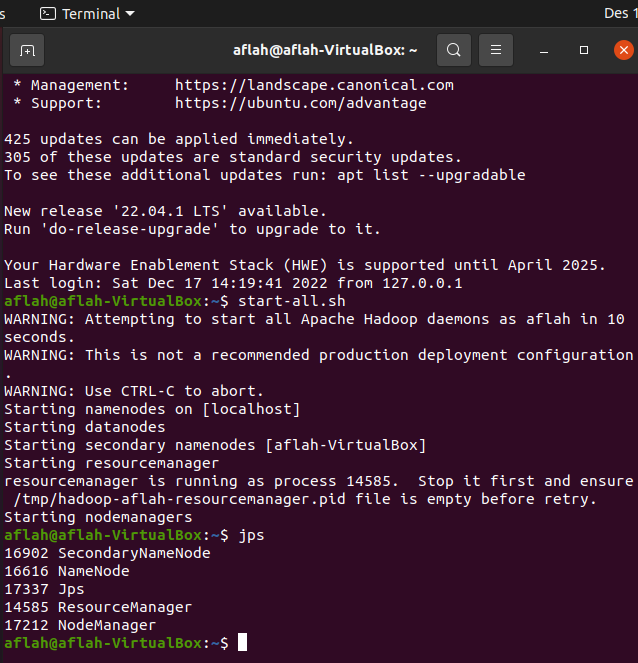
\includegraphics[width=\textwidth]
{FaizaYuwafiqi/jps}
\caption{hasil dari jps}
\label{gam:perkuliahan-25-11}
\end{figure}

\begin{figure}
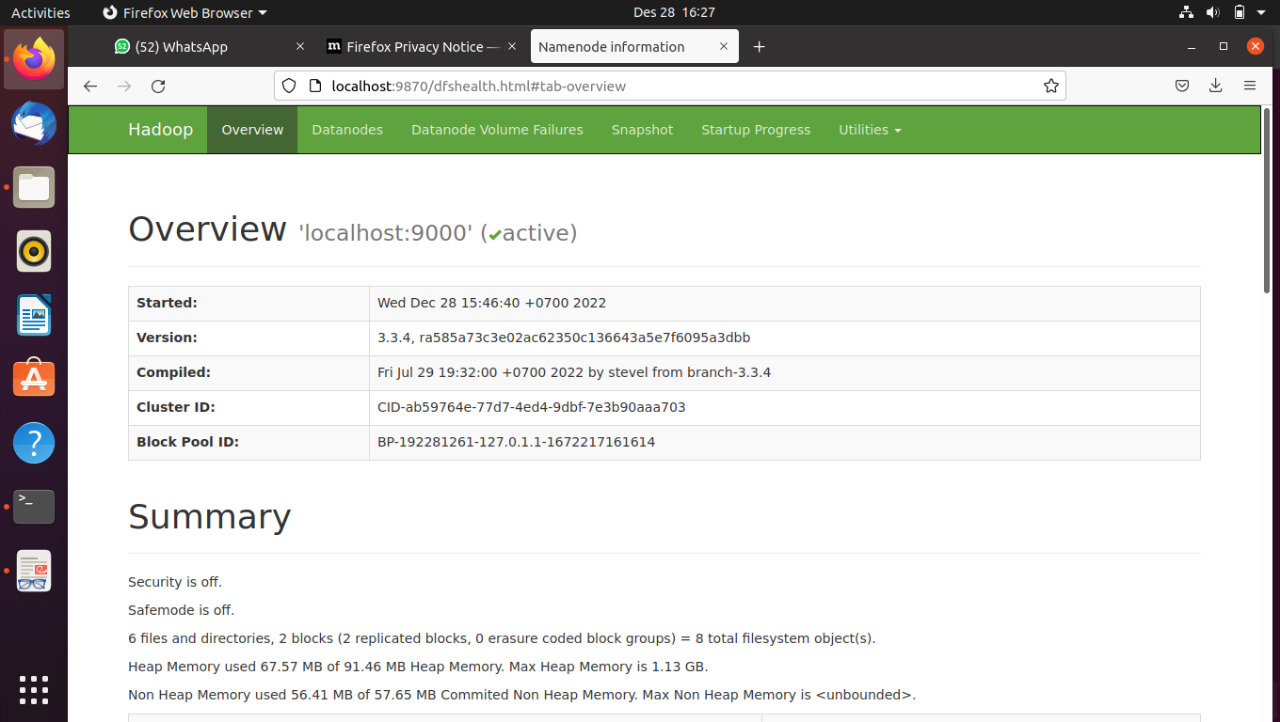
\includegraphics[width=\textwidth]
{FaizaYuwafiqi/localhost9870}
\caption{hasil dari localhost 9870}
\label{gam:perkuliahan-25-11}
\end{figure}

\newpage
\begin{figure}
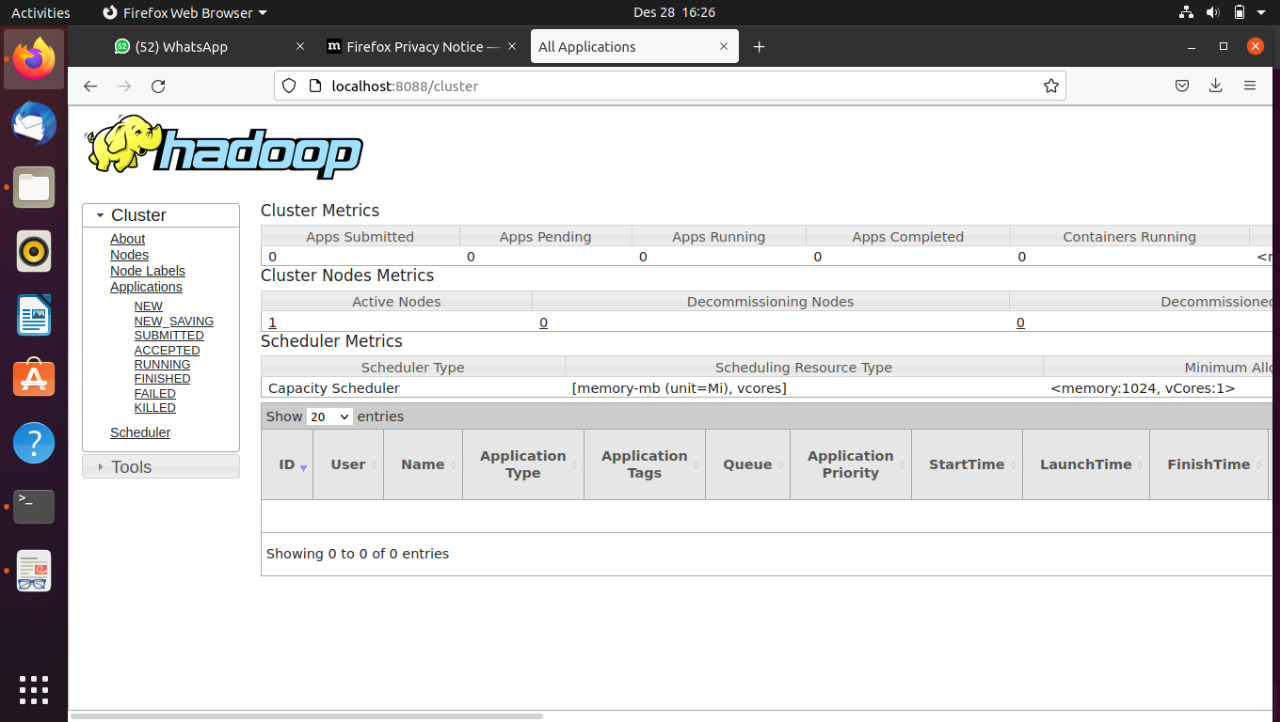
\includegraphics[width=\textwidth]
{FaizaYuwafiqi/localhost8088}

\caption{hasil dari localhost 8088}
\label{gam:perkuliahan-25-11}
\end{figure}

\end{enumerate}


\newday{\textbf{8 Desember 2022}}
\begin{enumerate}
\item Kendala dan Solusi
% jelaskan kendala dan penyebab yang dialami saat mengikuti praktikum serta solusi atau langkah-langkah yang telah dilakukan

\item Kesimpulan
% berikan kesimpulan dari praktikum yang telah dikerjkan

\end{enumerate}

\newday{\textbf{9 Desember 2022}}
\begin{enumerate}
\item Kendala dan Solusi
% jelaskan kendala dan penyebab yang dialami saat mengikuti praktikum serta solusi atau langkah-langkah yang telah dilakukan

\item Kesimpulan
% berikan kesimpulan dari praktikum yang telah dikerjkan

\end{enumerate}

\newday{\textbf{15 Desember 2022}- WordCount Bawaan Hadoop}
\begin{enumerate}
\item Kendala dan Solusi
\newline Kendala, masalahnya saat pengisian nano ada yang typo sehingga program lain tidak mau jalan.
\newline Solusi, memperbaiki typo pada nano dan program berhasil jalan

\item Kesimpulan
\newline harus lebih memperhatikan codingan yang diketik agar tidak terjadi typo dan program tidak mau jalan

\newpage
\begin{figure}
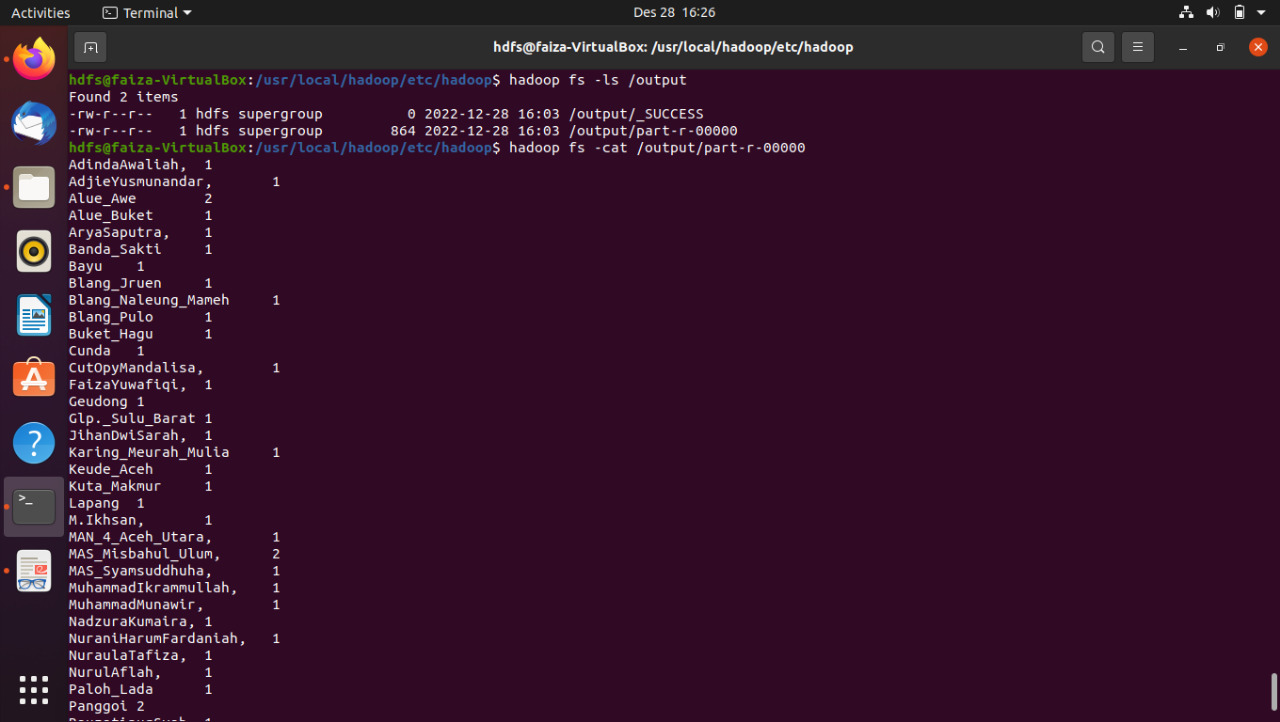
\includegraphics[width=\textwidth]
{FaizaYuwafiqi/6 dan 7 a}
\caption{hasil dari langkah 6 dan 7}
\label{gam:perkuliahan-25-11}
\end{figure}

\begin{figure}
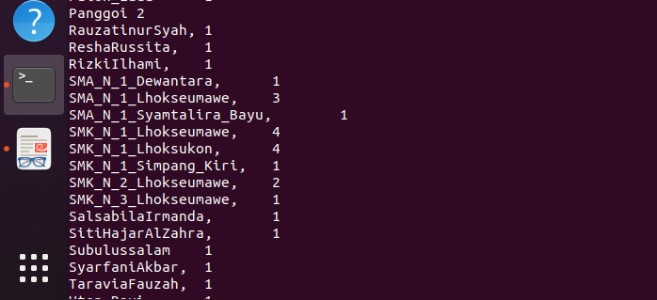
\includegraphics[width=\textwidth]
{FaizaYuwafiqi/6 dan 7 b}
\caption{sambungan hasil dari langkah 7}
\label{gam:perkuliahan-25-11}
\end{figure}

\end{enumerate}

\newday{\textbf{16 Desember 2022} -WordCount dengan Java}
\begin{enumerate}
\item Kendala dan Solusi
\newline Kendala, program tidak mau di compile karna ada penulisan yang typo dan tertinggal dalam nano.
\newline Solusi, memperbaiki isi nano

\item Kesimpulan
\newline beberapa kesalahan terjadi karena isi modul yang berubah, sehingga harus mencari modul lama yang memiliki codingan lengkap.

\newpage
\begin{figure}
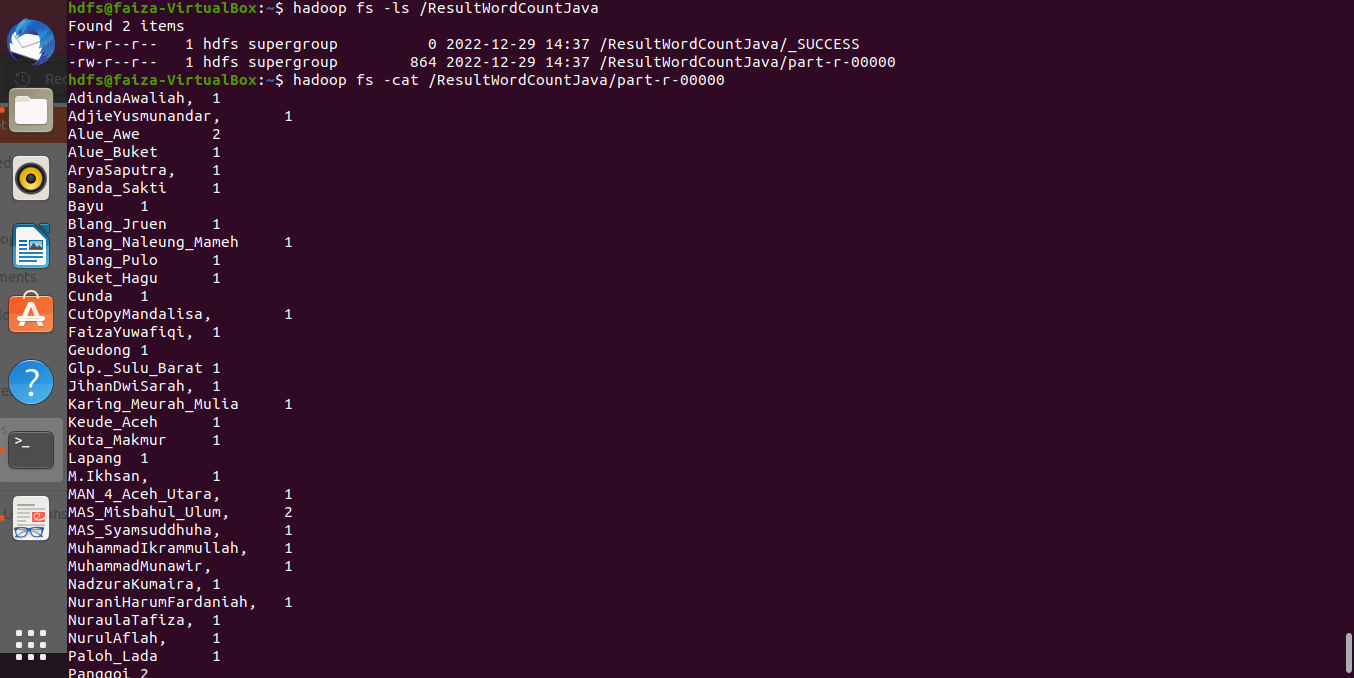
\includegraphics[width=\textwidth]
{FaizaYuwafiqi/9 dan 10 a}
\caption{hasil dari langkah 9 dan 10}
\label{gam:perkuliahan-25-11}
\end{figure}

\begin{figure}
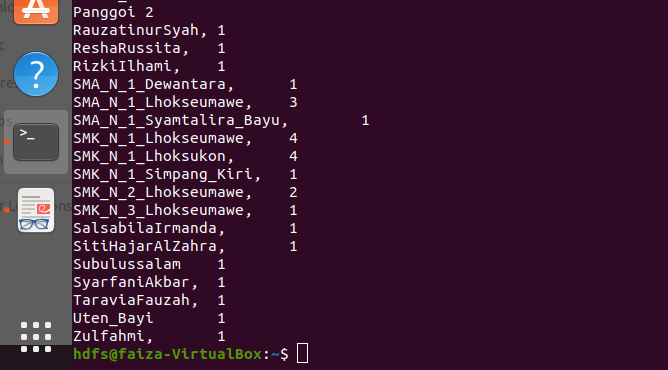
\includegraphics[width=\textwidth]
{FaizaYuwafiqi/10 b}
\caption{sambungan hasil dari langkah 10}
\label{gam:perkuliahan-25-11}
\end{figure}

\end{enumerate}

\newday{\textbf{22 Desember 2022}}
\begin{enumerate}
\item Kendala dan Solusi
\newline Pada saat melakukan instalasi tidak ada terjadi error

\item Kesimpulan
\newline instalasi berjalan lancar

\newpage
\begin{figure}
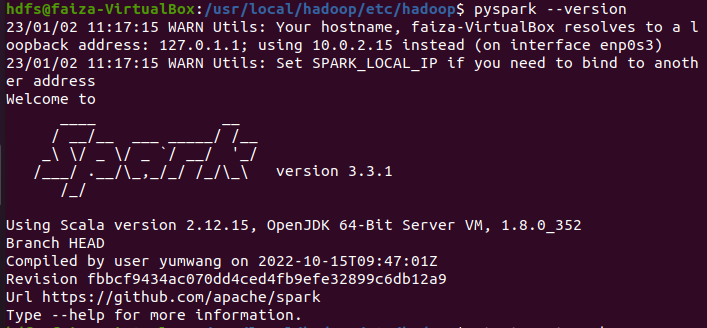
\includegraphics[width=\textwidth]
{FaizaYuwafiqi/pyspark}
\caption{hasil dari instalasi pyspark}
\label{gam:perkuliahan-25-11}
\end{figure}

\end{enumerate}

\newday{\textbf{23 Desember 2022}}
\begin{enumerate}
\item Kendala dan Solusi
pada saat proses wordcount dilakukan terdapat typo pada penulisan kata WordCount sehingga nano tidak tersimpan dengan benar

\item Kesimpulan
kesalahan tersebut telah diperbaiki

\newpage
\begin{figure}
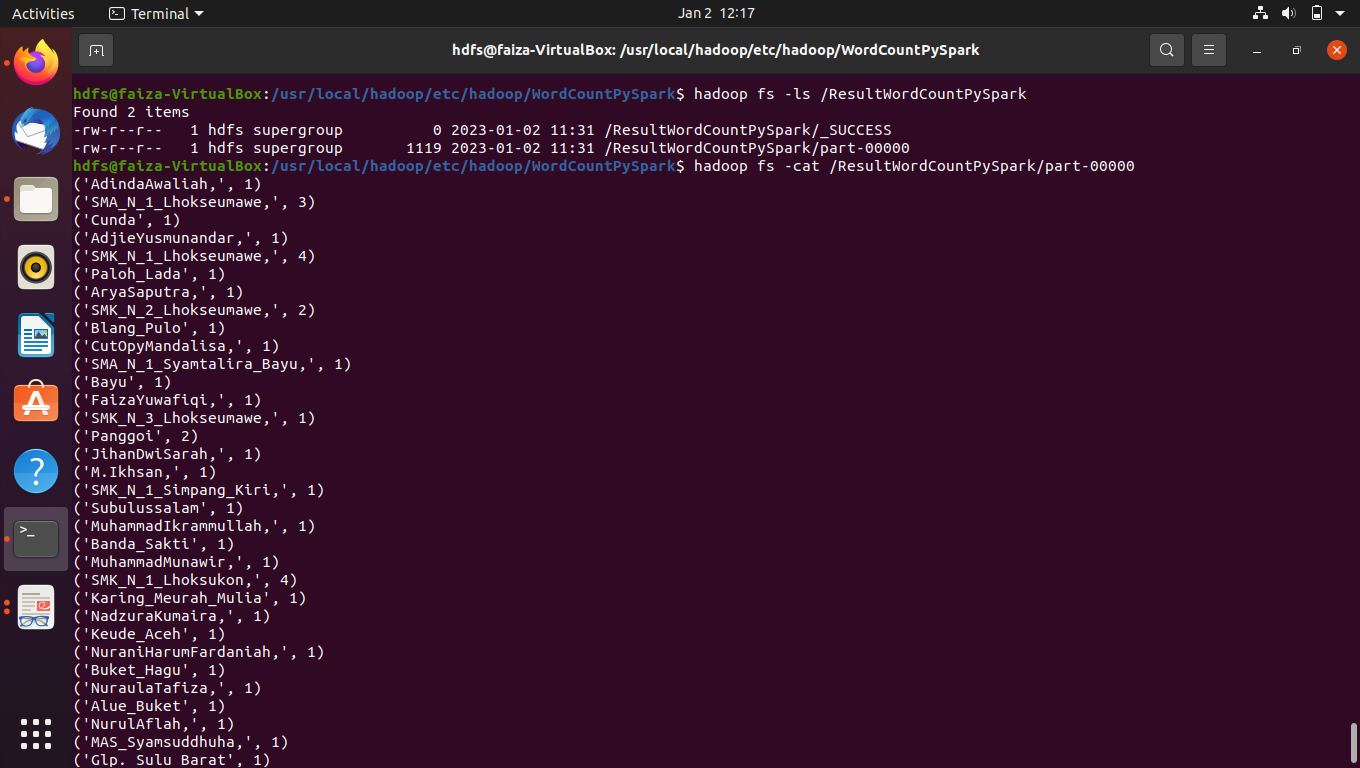
\includegraphics[width=\textwidth]
{FaizaYuwafiqi/wc pyspark}
\caption{hasil dari Wordcount Pyspark}
\label{gam:perkuliahan-25-11}
\end{figure}

\begin{figure}
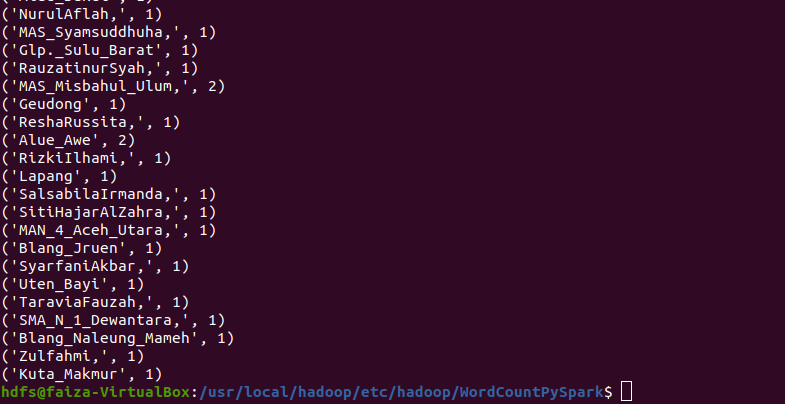
\includegraphics[width=\textwidth]
{FaizaYuwafiqi/wc pyspark 2}
\caption{sambungan hasil dari Wordcount Pyspark 2}
\label{gam:perkuliahan-25-11}
\end{figure}

\end{enumerate}

